\chapter{Characters}
\label{ch:characters}

\section{Player Characters}
A Player Character (PC) is your representation in the game. Your eyes, ears, touch, feel and smell in the imaginary world that you and your fellow players create.

On one hand the character is a collection of numbers which describe his/her characteristics, skills and magic spells that are written down on a character sheet.  This chapter will explain how you create these numbers, in a process known as Character Generation. But that is only half of what a character is.

The other half exists mainly in the imagination of the player, with perhaps some quick notes on the character sheet. This half is the personality of the character and other intangibles such as goals and past history. These are the things that you can’t express in cold hard numbers, which really bring the character to life and give the player guidelines on how the character acts and thinks.


\section{Character Generation}
Fantasy D100 character generation is a multi-step process and at each step the Player makes decisions about what their character is like at the beginning of their adventuring career. 

\subsection{Concept}
A character concept is a one sentence summing up of what the character is all about.

\begin{rpg-examplebox}
\begin{rpg-list}
\item Rurik is ``A determined and foolhardy warrior seeking excitement and adventure.''
\item Lura is ``A mysterious and elegant arcane magic user.''
\item Mancala is ``The illegitimate son of a murdered Noble, who survives through being a rogue.''
\item Abnon is ``A pious priest who smites evil and protects the innocent.''
\end{rpg-list}
\end{rpg-examplebox}

Having a clear concept of what you want your character to be like at the beginning of character generation guides the whole process as you make choices to generate the numbers that you will roll against during play.

For example, for Rurik it states clearly that he is a warrior, therefore when choosing skills Rurik puts points into Dodge and Unarmed combat, both skills that will be highly useful when he gets into a fight, rather than any of the Lores.

You are of course free to change the concept as you generate the character. Generally, as a rule, the stronger the character concept, the easier it is to create an interesting character.

%Your Gamemaster may ask you what your character concept is before you start Character Generation, to make sure that it fits in with the sort of game that he has prepared.  For example creating a warlike barbarian may not be a good idea for a game that is going to revolve around a series of magical mysteries where the characters will need strong investigative and magical skills.

%Comparing concepts with the other players before diving into character creation is strongly recommended. Your character will be part of an adventuring group that is made up of the other Player characters. These characters work together, even if they don’t like each other, towards a common goal of solving the mysteries and dilemmas thrown up by the Gamemaster during the adventures that they play through. The game is unlikely to be any fun if all the players have similar or near identical concepts, as compared with a game where the group is made up of characters with different concepts that can work together to create interesting role-playing opportunities.


\subsubsection{Step 1: Determine Concept}
In one sentence sum up what your character is all about. Use the guidelines above to give yourself ideas. Ask the other Players what their character concepts are to make sure the group has an interesting selection of characters.

Check with your Gamemaster that your character concept fits in with the type of game that the group is going to be playing.

%\begin{figure}[h]
%\begin{center}
%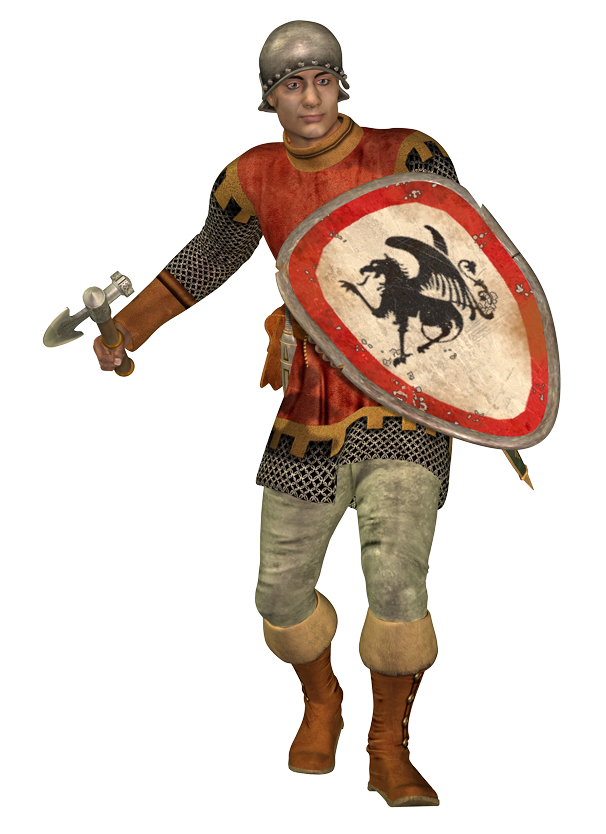
\includegraphics[scale=0.25]{img/colored/adventurer2.png}
%\end{center}
%\end{figure}

\subsection{Characteristics}
These are the primary building blocks of the character. All characters and creatures have seven characteristics, which give the basic information about the character’s physical, mental and spiritual capabilities.

As well as being useful indicators of how to roleplay the character (see below) they are the scores that skills are initially based upon. The characteristics are:

\begin{description}
	\item[Strength (STR):] A character’s brute force, Strength affects the amount of damage he deals, what weapons he can wield effectively, how much he can lift and so on. 
	\item[Constitution (CON):] A measure of the character’s health, Constitution affects how much damage he can sustain in combat, as well as his general resistance to disease and other illnesses.
	\item[Dexterity (DEX):] A character’s agility, co-ordination and speed of reaction, Dexterity aids him in many physical actions, including combat. 
	\item[Size (SIZ):] This is an indication of the character’s mass and, like Strength and Constitution, can affect the amount of damage a character can deal and how well he can absorb damage.
	\item[Intelligence (INT):] A character’s ability to think around problems, analyse information and memorise instructions. It is a very useful Characteristic for characters interested in becoming accomplished spellcasters. 
	\item[Power (POW):] Perhaps the most abstract Characteristic, Power is a measure of the character’s life force and the strength of his willpower. It is the basis of all extraordinary or supernatural powers (see Disciplines and Powers in Part II).
	\item[Charisma (CHA):] This quantifies a character’s attractiveness and leadership qualities. 
\end{description}


\subsubsection{Step 2: Generating Characteristics}
Each characteristic starts with a value of 8.  You next have thirty points to distribute amongst them. The maximum value of a characteristic during character generation is 18. You may also lower a characteristic to gain extra points. For example, reduce STR 8 to 6 to gain 2 points, but INT and SIZ have a minimum value of 7. Other characteristics have a minimum value of 3, although this indicates that the character has a severe disadvantage in this area. 

The Points method is better if you already have a clear idea of your character concept as it gives you precise control on the relative strength of each characteristic. You are not at the mercy of random dice rolls (see Random Characteristics optional rule) nor do you have to negotiate with your Gamemaster about switching the random rolls around so that the characteristic scores match your concept.

\begin{rpg-examplebox}
Rob is playing Rurik, who is a rough and ready warrior, and spends his 30 points in the following way.

	\stats[STR=18, CON=12, DEX=12, SIZ=16, INT=10, POW=8, CHA=10]

He adds ten, four, and eight to STR, CON and SIZ respectively to get a higher damage modifier and hit points total and for the ‘big bruiser’ element of the character concept, and four to  DEX since that determines when he acts in initiative and is the base for many important skills for warriors. Finally he adds two points to both INT and CHA, to make sure Rurik is average for Intelligence and sociability.  He chooses not to increase POW at character creation since he doesn’t really see Rurik as much of a magic user at the start of the game.
\end{rpg-examplebox}

%\subsubsection{Maximum Value of Characteristics}
For any race the maximum value of any characteristic is the maximum dice roll plus three. For Humans this is 21.

%\subsubsection{Extreme Characteristics}
One feature of the points buy system is that it tends to produce characters that are close to the average score, unless you choose to reduce one of your characteristics from the initial allocation of eight or leave it unmodified. By taking that approach you will have some weak characteristics, such as a DEX of 8 indicating that your character is a bit slow and clumsy, but you will also have a few strong characteristics, such as an INT of 18 which shows your character is a natural born genius. 

You can also end up with characters with high and low characteristics using the random method as well.

Such characters may at first glance look undesirable, on account of how base skills are affected, but actually they present good opportunities for roleplaying the flaws of the character, and actually makes the character more interesting as a result.

\vspace{3mm}
\begin{rpg-titlebox}{Random Characteristics}
Players can also roll for characteristics. For human characters roll 3D6 for STR, CON, DEX, POW and CHA and 2D6+6 for INT and SIZ. Reroll 1's to prevent very low scores.
\end{rpg-titlebox}


%\subsubsection{Using Characteristics in Roleplaying}
%As well as being numbers that are used to calculate the skills and attributes that influence the dice rolls that are made during the game, characteristics can also be used to give rough ideas as to what the character is like. The average human has scores between 10 and 11 in most characteristics, except Size and Intelligence which weigh in around 13. So a character with Strength of 16 will be of above average Strength and a toned physique.  A character with a Charisma of 7 is well below average, perhaps being shy or obnoxious and socially inept. 


\subsection{Attributes}
Attributes are a set of secondary scores that define the character’s potential to do and take physical damage, how quickly they move, and the amount of extraordinary or supernatural powers available to the character. Attributes are determined from the character’s characteristic scores. 

\begin{description}
	\item[Damage Modifier (DM):] The Damage Modifier applies whenever the character uses a melee or thrown weapon. It is used to show that bigger, stronger, characters deal out more damage than smaller, weaker characters. 
	\item[Hit Points (HP):] These determine how much damage the character can sustain before reaching unconsciousness or death.
	\item[Major Wound Level:] When the character takes this amount of damage in one go, they suffer a Major Wound. Major Wounds are injuries, such as a severed limb, broken ribcage or broken skull, which may render the character unconscious immediately and leave permanent affects if not healed by supernatural powers.
	\item[Power Points (PP):] These are used to activate any extraordinary or supernatural powers the character knows. If it is reduced to zero the character drops unconscious until they regain at least one point.
	\item[Movement Rate:] This is the amount in metres that a character can move in a five second Combat Round.
\end{description}

\begin{center}
\begin{table}
\caption{Damage Modifier table}
\label{tab:damage-modifier}
\begin{rpg-table}[|Y|Y|]
	\hline
    	\textbf{STR + SIZ}  & \textbf{Damage Modifier}\\
	\hline
   	1-10   & -1D6\\
   	11-15  & -1D4\\
   	16-25  & +0\\
   	26-30  & +1D4\\
   	31-45  & +1D6\\
   	46-60  & +2D6\\
   	61-75  & +3D6\\
   	Every additional +15  & +1D6\\
	\hline
\end{rpg-table}
\end{table}
\end{center}


\subsubsection{Step 3: Determine Attributes}
To work out your character’s Damage Modifier, add Strength and Size together and look at table~\ref{tab:damage-modifier}.

Hit Points equal Size plus Constitution divided by 2, rounded up. 

Major Wound Level is equal to Total Hit Points divided by two, rounded up.

The character’s starting Power Points will be equal to the character’s POW.

Human characters have a Movement rate of 15 metres.

\vspace{3mm}
\begin{rpg-titlebox}{Rounding}
	Numbers in Fantasy D100 are always rounded to the nearest whole number. Always round up from 0.5 and round down from below 0.5.  For example 4.1 becomes 4, while 5.5 becomes 6.
\end{rpg-titlebox}

\subsection{Skills}
Skills are things that the character can do. They represent very specific areas of expertise and when the skill is used in play the percentage value of the skill is rolled against using a D100 to work out if a character successfully completes a task in the game.  A roll equal to or less than the skill percentage usually indicates that the skill has been used successfully.

\begin{rpg-examplebox}
	Rurik has a Dodge of 52\%, which means that in combat he has to roll 52 or under on D100 to avoid the incoming blows of his opponent.
\end{rpg-examplebox}

Table~\ref{tab:skill-and-expertise} translates the skill percentage into a real world description of the level of expertise.
\begin{table}
\caption{Skill and Expertise}
\label{tab:skill-and-expertise}
\begin{rpg-table}[|l|c|X|]
	\hline
	\textbf{Skill}  & \textbf{Expertise} & \textbf{Description}\\
	\hline
	0-25\%   & Novice & Someone with virtually no experience with the skill.\\
	26-50\%  & Apprentice & Someone who is learning the skill.\\
	51-75\%  & Veteran & Someone who regularly uses the skill as part of their everyday life.\\
	76-99\%  & Expert & A local expert with the skill, who can perform it under most conditions with ease and elegance.\\
	100+     & Master & The acknowledged best in that skill, and regularly performs the impossible in extremely difficult conditions.\\
	\hline
\end{rpg-table}
\end{table}

From looking at the above table you can see that Rurik with his Dodge of 52\% is quite proficient, having an expertise level of Veteran, probably from being in actual combat on several occasions and learning by necessity to get out of the way of weapon attacks.

\subsubsection{Skill Lists}
The following tables lists all the skills that every character possesses and the Characteristics used to determine the skill’s base score. The tables also give each skill a brief description of what the skill does, but a fuller description is given in the Skills chapter. Skills are grouped into categories for easy reference:

\begin{description}
	\item[Resistances] are skills that get the character out of harms way.
	\item[Combat skills] measure the characters skills in physical violence.
	\item[Knowledge skills] measure the intellectual skills of the character.
	\item[Practical skills] measure the characters’ ability of performing a variety of everyday and specialist tasks.
%	\item[Magic skills] cover either casting magic or knowledge of religious practices.
\end{description}

Some skills like Lore (Type), Craft (Type) and Culture (Other) all have a descriptor in brackets after the main skill name. 
This denotes that at time of points allocation the player must decide what Type or Other is. For example Lore (Type) could be Lore (Heraldry) or Lore (Astronomy).


\begin{center}
\begin{table}
\caption{Resistances}
\label{tab:resistances}
\begin{rpg-table}[|l|c|X|]
	\hline
	\textbf{Skill}  & \textbf{Base} & \textbf{Description}\\
	\hline
	Dodge       & DEX+10  & Gets you out of the way of physical threats, such as an incoming axe or dragon breath.\\
	Persistence & POW+10  & Is a measure of your character’s willpower and resistance against hostile magic and is also rolled to resist attempts to influence the character against their will.\\
	Resilience  & CON+POW & Is a measure of your character’s health and their ability to survive exposure, hunger and thirst. It is also their chance to resist the effects of diseases.\\
	\hline
\end{rpg-table}
\end{table}
\end{center}

It’s worth putting the majority of your points into Dodge if you are going down the route of the Warrior with your character. If you are thinking more of a magic using character, Persistence is probably more appropriate. Resilience is good for hardy characters that can shrug off disease and stay conscious when they take damage.


\begin{center}
\begin{table}
\caption{Combat Skills}
\label{tab:resistances}
\begin{rpg-table}[|p{1.5cm}|c|X|]
	\hline
	\textbf{Skill}  & \textbf{Base} & \textbf{Description}\\
	\hline
	Close Combat    & DEX+STR & A character’s skill with melee weapons, such as swords, axes, daggers, spears and shields.\\
	Ranged Combat   & DEX+INT & A character’s skill with missile and thrown weapons.\\
	Unarmed Combat  & DEX+STR & A character’s skill with natural weapons such as bite, fist, kick, grapple and claws.\\
	\hline
\end{rpg-table}
\end{table}
\end{center}

It goes without saying that all these skills are appropriate for characters who want to be warriors.  A few points however in either close or unarmed combat are useful even for non-combative characters since these skills can be used for self-defence.


\begin{center}
\begin{table}
\caption{Knowledge Skills}
\label{tab:resistances}
\begin{rpg-table}[|l|c|X|]
	\hline
	\textbf{Skill}  & \textbf{Base} & \textbf{Description}\\
	\hline
	Culture (Own)    & INT+10 & What a character knows about the history, politics, geography of their own land and society.\\
	Language (Own)   & INT+50 & How fluent a character is at speaking and potentially reading and writing their own language.\\
	Natural Lore     & INT+10 & Predicting the weather, recognizing and caring for animals and plants, geology and survival in the natural world.\\
	Culture (Other)  & INT    & What a character knows about the history, politics and geography of a foreign land.\\
	Language (Other) & INT    & How fluent a character is at speaking and potentially reading and writing a foreign language.\\
	Lore (Type)      & INT    & Other specialist knowledge skills, such as Lore (Herbalist), Lore (Heraldry) not covered by the above.\\
	\hline
\end{rpg-table}
\end{table}
\end{center}


Knowledge skills are good for characters that are sages or scholars and who make their living from obscure information that other people do not have the time to learn. Culture (other) and Language (other) are also useful to characters whose abilities revolve around communications, such as merchants and diplomats.

\begin{center}
\begin{table}
\caption{Practical Skills}
\label{tab:resistances}
\begin{rpg-table}[|p{1.8cm}|c|X|]
	\hline
	\textbf{Skill}  & \textbf{Base} & \textbf{Description}\\
	\hline
	Athletics           & DEX+STR & This skill measures the characters's ability at running, lifting, jumping, swimming and climbing.\\
	Craft               & INT+10  & This skill allows you to make things, such as pots, weapons, and buildings.\\
	Deception           & DEX+INT & Stealth, hiding and picking pockets are all handled by this skill.\\
	Driving	            & DEX+INT & This skill covers ancient-medieval period vehicles such as carts, chariots and wagons.\\
	Engineering         & INT+10  & Large scale construction and siege engines are covered by this skill.\\
	Healing             & INT+10  & Healing wounds and treating disease using first aid and surgery.\\
	Influence           & CHA+10  & This skill is used when the character wants to persuade another to do something against their normal interests.\\
	Mechanisms          & DEX+INT & Locks and anything with complex moving parts are covered by this skill.\\
	Perception          & INT+POW & Used to spot hidden objects and spot small details in the character’s environment.\\
	Performance         & CHA+10  & Acting, playing instruments, dancing and singing are all covered by this skill.\\
	%Relationship (Type) & CHA+10  & An optional skill that shows the strengh of a character’s bond with a non-player character or group of non-player characters.\\
	Riding              & DEX+POW & Used when trying tricky manoeuvres using beasts of burden, such as horses, camels and more fantastic beasts such as hippogriffs.\\
	Sailing             & DEX+INT & This skill covers the use of ships and boats.\\
	Streetwise          & CHA+POW & How well the character operates in a city environment. Used to find out information and navigate around the streets and find a fence for stolen goods are all covered by this skill.\\
	Trade               & INT+10  & This is the skill used by merchants and traders to value and sell goods.\\
	%Wealth              & INT+CHA & An optional skill that measures a character’s ability to manage their resources.\\
	\hline
\end{rpg-table}
\end{table}
\end{center}

On the face of it, it is tempting to see the Practical category as a big grab bag of miscellaneous skills. However it is worth spending some points on one to three of the skills, even if you want to be a big muscled warrior.  These skills allow the character to do things in game, and Athletics, Influence and Perception get called upon reasonably frequently. Also if your character’s concept is that of a rogue Deception, Mechanisms and Streetwise also deserve some points. If your character is someone who makes stuff, Craft and Engineering are skills to increase. If your character has a background of entertaining people Performance is a skill to pick. If your character concept is any form of merchant Trade is a must buy.

%Magic is explained below, in Step 5, but for now just note that the three types of skill relate to the three types of magic.

%\begin{center}
%\header{Magic Skills}
%	\begin{rpg-table}[|l|c|X|]
%	\hline
%	\textbf{Skill}  & \textbf{Base} & \textbf{Description}\\
%	\hline
%	Battle Mgic     & POW x 3 & This skill allows you to use basic personal magic.\\
%	Arcane Magic          & INT     & This skill is used to cast and manipulate sorcery spells. For the non-magician it is your chance to use talismans and scrolls and other sorcerers’ items.\\
%	Religion         & INT+10  & Most characters will be at least ‘lay’ members of the religion local to them, taking a passing interest in its mythology and rituals. For more devoted characters this skill is the key to advancement in the religion’s hierarchy.\\
%	%Religion (Other) & INT     & This skill covers the knowledge of another religion, where other is the name of that religion.\\
%	\hline
%\end{rpg-table}
%\end{center}


\subsubsection{Step 4: Calculate Skills}
For each skill calculate the starting skill value, the base score, from the calculation provided. Then write it down on the character sheet next to the skill.  

During character generation the player gets a pool of points to spend on each group of skills. Distribute points between the skills, with a limit of no more than 30 to be allocated to any one skill.

\begin{rpg-table}[|l|X|]
	\hline
	Resistances   & Spend 50 points between the three skills.\\
	Combat        & Spend 50 points between the three skills.\\
	Knowledge     & Spend 50 points between the skills.\\
	Practical     & Spend 75 points between skills.\\
	\hline
\end{rpg-table}

For Players that want a more scholarly character they can reduce Combat points to increase Knowledge points at a 1:2 ratio; thus for 10 Combat points a character can get 20 additional Knowledge points. However, no skill can be increased by more than 30 points during character creation.


\subsection{Special Training}
Player Characters are extraordinary. On top of them being above average they may also have special training. This can manifest in improved skills or characteristic or even focusing in specific Disciplines. A Discipline may represent training in advanced combat techniques or magic powers or anything extraordinary or supernatural.


\subsubsection{Step 5: Select Disciplines and Powers}
Each character begins play with six Improvement Points (see page~\pageref{ssec:improvement-points}) that allow players to further improve in skills or even acquire new Disciplines. For choices of Disciplines and their Powers consult the chapters in Part II.

\subsection{Equipment}
Each character typically starts off with some money and the tools of their trade.

\subsubsection{Step 6: Starting cash and Equipment}
Starting cash is 4D6 x 10 in Silver Pieces. In addition each character starts out with one of the two arms and armour packages below.

\begin{rpg-list}
	\item Leather armour, ranged weapon, close combat 2H weapon and dagger. 
	\item Leather armour, shield, ranged weapon, close combat 1H weapon and dagger.
\end{rpg-list}

All characters also start out with the following equipment: backpack, rope, two weeks worth of traveling provisions, flint and tinder, waterskin.

Further information about equipment and game economics is given in the chapter~\ref{ch:equipment}. Your Gamemaster may allow you to buy additional equipment before the game starts from the character’s starting cash.

\subsection{Finishing Touches}
By this stage all the hard decisions on making your character are over.  All that remains is to note down a few numbers on the character sheet and ponder about the character’s background and motives.

\subsubsection{Age}
Human characters start out at any age between 18 and 28. To randomly determine this, roll 2D6 and add 16. 

\subsubsection{Hero Points}
Every character starts with two Hero Points. Hero points are what distinguishes the player character from the normal stay at home type folk. They allow the player character to:

\begin{rpg-list}
	\item Re-roll any failed dice roll.
	\item Downgrade a Major Wound to a normal wound. Full damage is applied to the character's Hit Points, but do not suffer the messy effects of a major wound.
	\item Avoid character death. If the character’s Hit Points are reduced to zero or less, instead of dying the character is merely unconscious. The character remains in such a state until the combat is over at which point they awaken with one Hit Point.
	\item Any other bonus or benefit to accomplish something at the Gamemaster discretion. This can include editing the plot. More than one Hero Points may be used (from multiple characters if desired) and something in favour of the players will happen. The Gamemaster may allow the players to choose the plot edit. An example of an one point edit would be a guard to forget to lock the cell that the characters are imprisoned. An example of a five points edit would be a dragon to happen to attack the castle giving the opportunity to escape!
\end{rpg-list}

Once Hero Points are spent they are gone. The Gamemaster awards Hero Points at the end of the game session for moments of outstanding heroic play or for significant achievements.

\subsubsection{Background, Appearance and Personality}
A background is useful not only to give the character a history before the game starts but also as a way of noting all the intangible elements of the character’s personality. 

Even if you don’t create a fully written up background it is worth making a mental note of what the character is like as a person and roughly what their background is previous to play, as well as visualizing what they actually look like. 

\subsubsection{Step 7: Finishing Touches}
Note down Hero Points and age. Hero Points start at 2 for all player characters regardless of race. Age for humans is 18-28 (2D6+16) years old.

Finally, if you want to include a background narrative do this now and if you haven’t done so already write the character’s name on the character sheet.


\section{Improving Characters}

\subsection{Improvement Points}
\label{ssec:improvement-points}
Through their adventures character will earn experience, awarded by the Gamemaster as a reward for certain achievements. This experience, called Improvement Points, will allow characters to improve.

\subsubsection{Improving Skills}
A player can choose to spend one Improvement Point to increase one or two skills.
Select one or two skills that are below 75\% to be increased and split +5\% points to those skills. Skills from 76\% to 99\% are increased by only 2\% for each IP and skills at Mastery level, i.e. 100\% or more, require one IP for a +2\% in a single skill.
There is no limit to the score a skill can reach. 

\subsubsection{Improving Characteristics}
A player can choose to spend three Improvement Points to increase one Characteristic by one point. 
SIZ may never be increased using Improvement Points. 
The maximum a human character can increase a Characteristic to is 21. For non-humans, the maximum for a Characteristic is equal to the maximum possible starting score for the Characteristic plus three.

\subsubsection{Acquiring Disciplines and Powers}
A player can choose to spend Improvement Points to acquire new Disciplines. Consult the appropriate Discipline chapter for details of how many points are required get the Discipline as well as how much is required to get each Power within it.

\subsection{Practice \& Research}
The characters may often experience long stretches of downtime between adventures. This is quite normal. Group members may need to heal from wounds suffered during the last adventure, the characters may engage in some activity that takes time, or life may simply return to normal until the next danger to face the player characters appears.

During such downtime the characters may improve their characters. The players might actually request downtime between adventures to learn new skills and it is up to the Gamemaster to determine if this is appropriate.  
For each three month period of practice or research a character may gain 1 Improvement Point. 


